\documentclass[tikz,border=10pt]{standalone}
\usepackage{tikz}
\usetikzlibrary{arrows.meta,calc}

\definecolor{figazul}{RGB}{2,132,199}
\definecolor{figrojo}{RGB}{220,38,38}
\definecolor{figverde}{RGB}{22,163,74}

\begin{document}
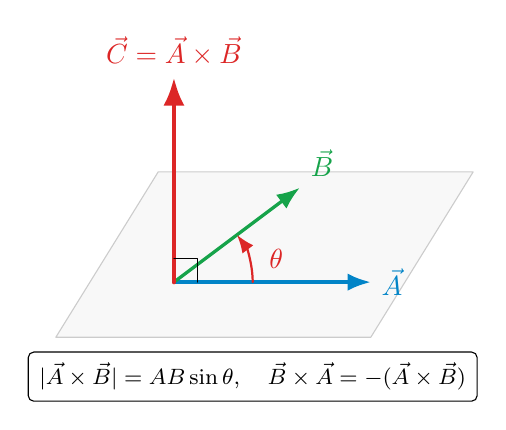
\begin{tikzpicture}[>=Latex, line cap=round, line join=round]
  % Plano base en perspectiva
  \fill[gray!10, opacity=0.5] (-0.5,-0.5) -- (3.5,-0.5) -- (4.8,1.6) -- (0.8,1.6) -- cycle;
  \draw[gray!40, thin] (-0.5,-0.5) -- (3.5,-0.5) -- (4.8,1.6) -- (0.8,1.6) -- cycle;

  % Origen
  \coordinate (O) at (1.0, 0.2);

  % Vector A (en plano, hacia la derecha)
  \draw[->, very thick, color=figazul] (O) -- ($(O) + (2.5, 0)$) node[right, color=figazul] {$\vec{A}$};
  % Vector B (en plano, hacia arriba y derecha)
  \draw[->, very thick, color=figverde] (O) -- ($(O) + (1.6, 1.2)$) node[above right, color=figverde] {$\vec{B}$};

  % Vector C = A x B (perpendicular al plano, hacia arriba)
  \draw[->, ultra thick, color=figrojo] (O) -- ($(O) + (0, 2.6)$) node[above, color=figrojo] {$\vec{C} = \vec{A} \times \vec{B}$};

  % Ángulo theta entre A y B
  \draw[->, thick, color=figrojo] ($(O) + (1.0, 0)$) arc (0:37:1.0);
  \node[color=figrojo] at ($(O) + (1.3, 0.3)$) {$\theta$};

  % Símbolo de ángulo recto entre C y plano
  \draw[thin] ($(O) + (0, 0.3)$) -- ($(O) + (0.3, 0.3)$) -- ($(O) + (0.3, 0)$);

  % Cartel explicativo
  \node[draw, rounded corners=2pt, inner sep=4pt, fill=white, fill opacity=0.9, text opacity=1, font=\footnotesize] at (2.0, -1.0)
    {$|\vec{A} \times \vec{B}| = AB\sin\theta, \quad \vec{B} \times \vec{A} = -(\vec{A} \times \vec{B})$};
\end{tikzpicture}
\end{document}
